\documentclass{article}
\usepackage[UTF8]{ctex}
\usepackage{multicol}
\usepackage{amsmath}
\usepackage{chngpage}
\usepackage{indentfirst}
\usepackage{geometry}
\usepackage{graphicx}
\geometry{left=2.0cm,right=2.0cm,top=3cm,bottom=3cm}
\begin{document}
\setlength{\parindent}{2em}
\title{RISCV CPU report}
\author{杨雨欢 517030910393}
\maketitle
\section{任务介绍}
本作业是本学期的大作业,主要目标是使用Verilog(或其它HDL)完成一
个能实现32 位RISC-V 指令集整数部分用户级别实模式的CPU。\\
\indent
RISC-V 是UC Berkeley 设计的开源指令集架构,在设计上属于精简指令集。\\
\indent
该代码已通过不带数据的模拟测试。
\section{代码思路}
代码采用了经典的五级流水架构,将执行分为取指令(Instruction Fetch)、译码(Instruction Decode),执行(Execution),内存访问(Memory),写回(Write Back)五个阶段,并对可能出现的hazard进行了一定的处理
\subsection{data hazard的处理}
针对data hazard实现了全部的数据forwarding,使得ID阶段能够拿到前一条或两条指令在EXE或MEM阶段做好的运算结果,从而避免RAW类型的hazard。\\
\indent
不过,即使实现了所有的data fawarding,针对涉及load指令的RAW data hazard,仍需暂停一个周期。
\subsection{structual hazard的处理}
由于只有一个内存读/写接口,当进行MEM操作时不能读取指令,会出现structural hazard。本人采用了暂停来避免structural hazard——当出现MEM操作时,MEM及其之前的模块全部暂停直至内存读取结束。
\subsection{control hazard的处理}
对于由分支引起的control hazard,不暂停流水线,pc在碰到branch语句之后不做任何处理,正常取出下一条指令,即是预测永远不跳转策略。当branch语句进入EX阶段时,如果发现需要跳转,则更改pc值,并刷新EX之前的两个缓冲区,以保证正确性。
\section{主题模块简介}
\paragraph{pc-reg}用于实现pc寄存器,给出需要读取的指令地址,每个时钟周期向后移动,当流水线暂停时保持不变。
\paragraph{mem-buffer}进行有关内存操作的控制模块。收集来自IF阶段和MEM阶段的读取内存请求,根据情况向控制器发送流水线暂停信号,通过CPU的读写接口与内存进行交互,并向IF和MEM阶段返回读写内存答复。
\paragraph{ctrl}用于控制流水线的暂停。得到来自mem buffer请求暂停的信号后,根据情况向pc及IF-ID、ID-EX、 EX-MEM、MEM-WB四个缓冲区发出控制信号,从而实现流水线的暂停。
\paragraph{regfile}用于实现32个寄存器,拥有一个写入接口和两个读出接口,写入采用时序电路,而读出采用逻辑电路,能够保证同一周期先写后读的正确性。
\paragraph{五级流水基本模块}IF、ID、EX、MEM、分别实现了流水线的前四级功能。同时在基本模块两两之间设立了缓冲区,用于流水线的控制。WB阶段直接通过缓冲区向寄存器连线完成,没有特别的模块。
\section{进一步改进方向}
由于时间原因,未能进行更进一步的性能改进,现将改进方案简要叙述如下:
\subsection{cache的实现}
由于内存读取是目前制约性能的最大因素,加入cache应该可以很大地弥补内存的不足。拟采用直接映射cache,并将数据和指令分开实现成两个cache,这样不但可以极大地降低指令的miss rate,还能够一定地消除由于内存操作而导致的structural hazard。
\subsection{分支预测的优化}
使用简单的两位分支预测器就可以显著提高分支预测的正确率,进而提升流水线的性能。更进一步地,可以结合指令cache,实现BTB(Branch Target Buffer)结构,在IF阶段就能够给出预测并指定pc的位置,从而消除由于分支而造成的流水线暂停,提升性能。
\section{附录}
\begin{figure}[ht]
\centering
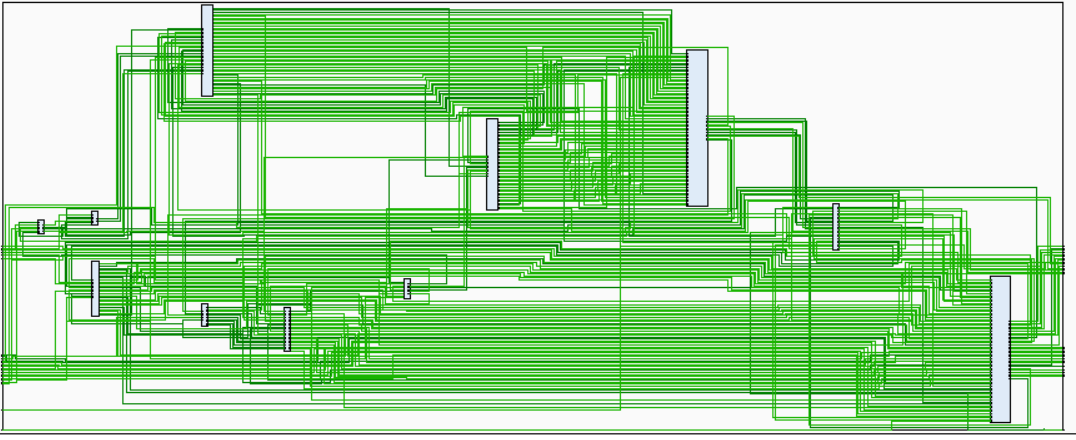
\includegraphics[scale=0.4]{cpu.png}
\caption{cpu内部连线图}
\end{figure}
\begin{figure}[ht]
\centering
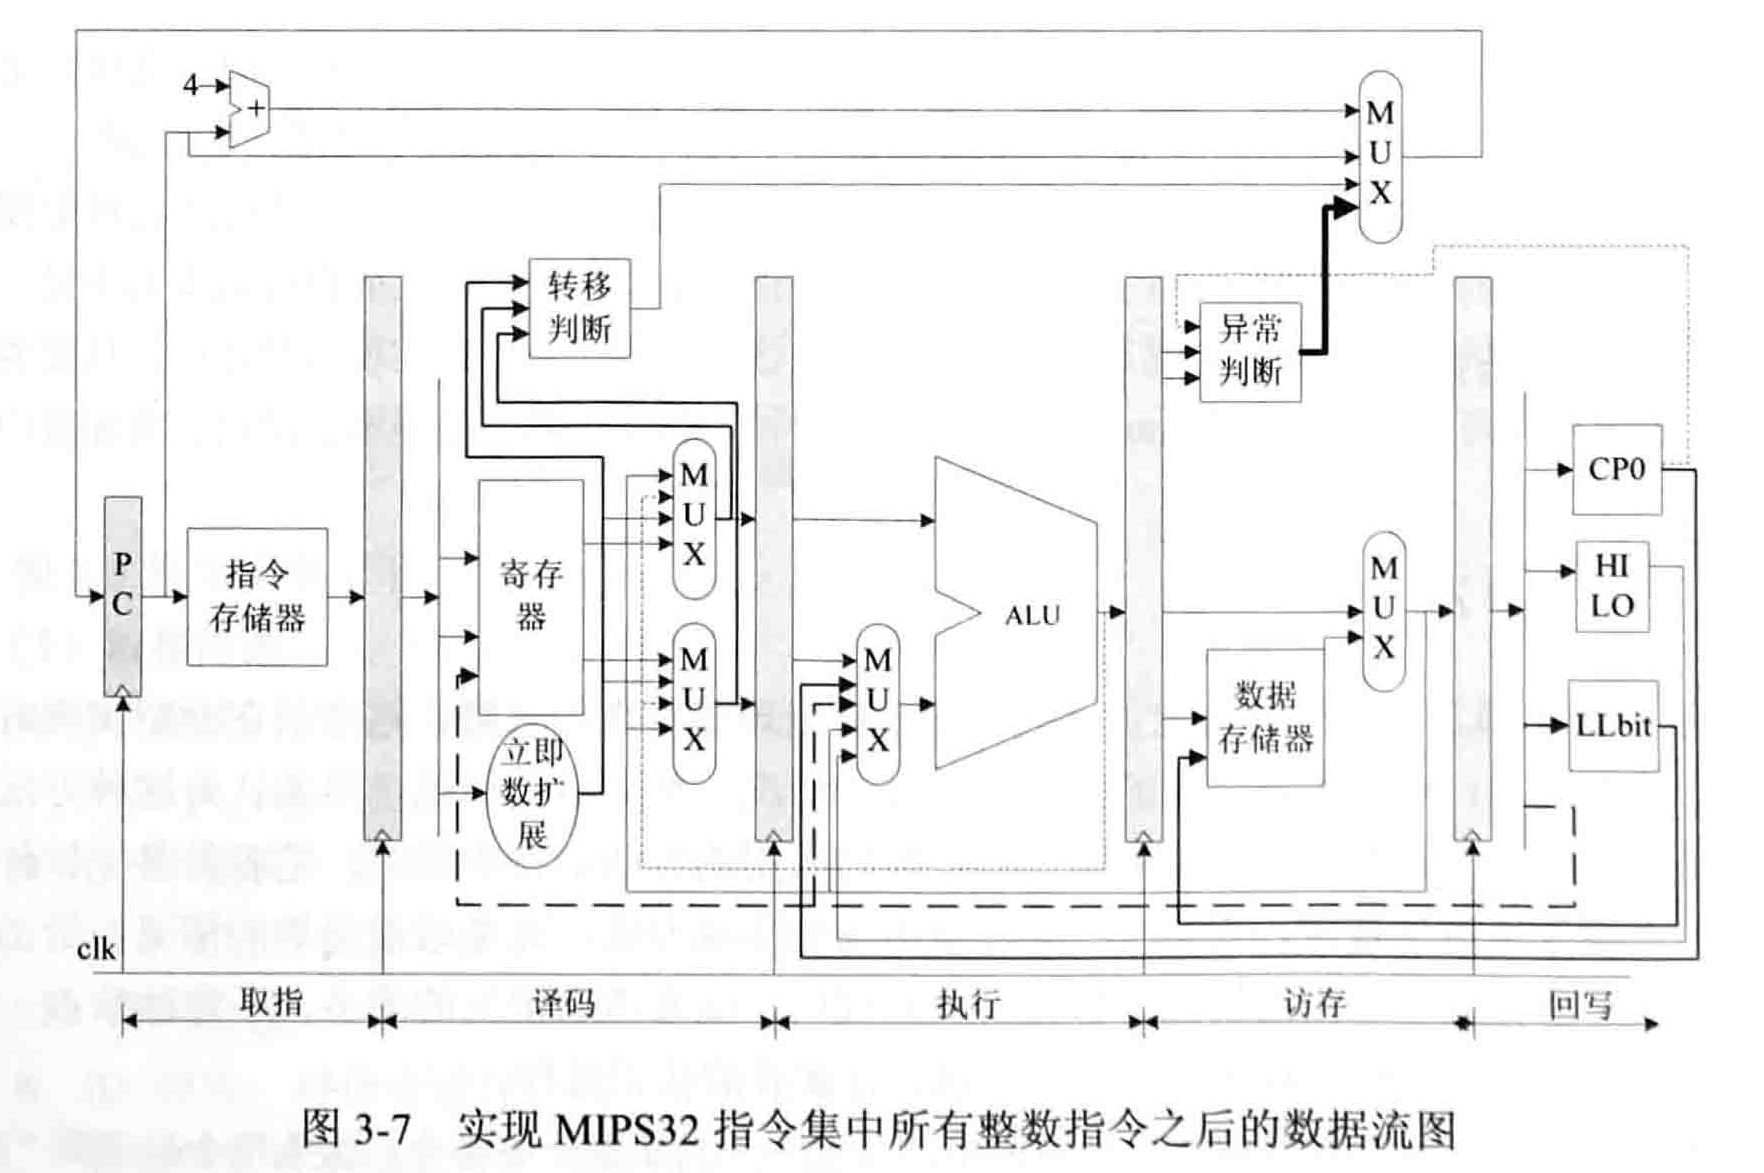
\includegraphics[scale=0.4]{structure.png}
\caption{cpu结构模型,图来自《自己动手写cpu》}
\end{figure}
\section{鸣谢}
在完成过程中,《自己动手写cpu》给了我极大的帮助。\\
\indent
同时也感谢给予我帮助的张文涛同学、杨孟天同学和钱苏澄同学。
\end{document}